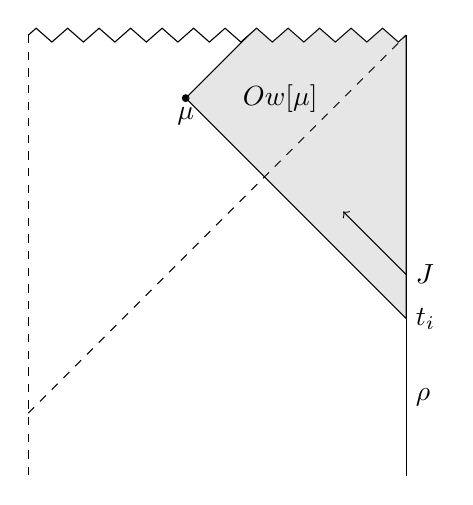
\begin{tikzpicture}[scale=0.8]

  \coordinate (bl) at (0, 0);
  \coordinate (tl) at (0, 7);
  \coordinate (tr) at (6, 7);
  \coordinate (br) at (6, 0);
  \coordinate (owtl) at (4.5, 8);
  \coordinate (owtr) at (6 ,8);
  \coordinate (iwtr) at (0.5, 8);
  \coordinate (iwtl) at (0, 8.5);
  \coordinate (iwbl) at (0, 3.5);
  \coordinate[label=right:$t_i$] (owbr) at (6, 2.5);
  \coordinate (ehb) at (0, 1);
  \coordinate (iwlab) at (1,6);
  \coordinate (owlab) at (4,6);

  \coordinate (sig) at (2.5, 6);


  \begin{scope}[decoration={zigzag, segment length=0.4cm}]


    \draw[decorate] (tr) to (tl);
    \draw[dashed] (tl) to (bl);
    \draw[dashed] (ehb) to (tr);
    \draw (tr) to (br);

    \path[clip] (tl) decorate {to (tr)} to (br) to (bl) -- cycle;

    \coordinate[label=below:$\mu$] (sig) at (2.5, 6);
    \node at (sig)[circle,fill,inner sep=1pt]{};
    \draw[fill=gray, fill opacity=0.2] (sig) to (owtl) to (owtr) to (owbr) to (sig);
    \node at (owlab) {$Ow[\mu]$};



  \end{scope} 

  \onslide<2->{
    \coordinate[label=right:$\rho$] (rholab) at (6, 1.25);
  }

  \onslide<3->{
    \draw[->] (6, 3.2) to (5, 4.2);
    \coordinate[label=right:$J$] (0) at (6,3.2);
  }



\end{tikzpicture}
